\documentclass[conference]{IEEEtran}
\usepackage{cite}
\usepackage{amsmath}
\usepackage{graphicx}
\usepackage{booktabs}
\usepackage{multirow}
\usepackage{url}
\usepackage{xcolor}

% 说明：所有数值均来自 experiment/results/trees.csv；写作时严禁占位数字。
\newcommand{\tbd}[1]{\textcolor{red}{[待填：#1]}}

\begin{document}

\title{Can a Local LLM Generate Branching NPC Dialogue Trees?\\
An Empirical Study of Depth--Quality Trade-offs}

\author{\IEEEauthorblockN{Anonymous Submission}
\IEEEauthorblockA{Software B Course Project, Fall 2026}}

\maketitle

\begin{abstract}
Branching dialogue trees are a core authoring cost in role-playing games, and large language
models (LLMs) are increasingly proposed as a way to generate them automatically. Yet it remains
unclear whether a small, locally deployable model can keep a character coherent as the tree grows
deeper. We study this question with a controlled experiment: a local 1.5B-parameter model is given
the same world setting and NPC profile, and asked to produce binary dialogue trees of depth
$d\in\{2,4,6\}$ (3, 15 and 63 nodes respectively). We compare prompt-only generation against a
LoRA adapter trained on a programmatically synthesised, structure-aligned corpus, and evaluate the
outputs with (i) deterministic structural and stylistic metrics and (ii) a three-scale rubric
(consistency, persona stability, choice meaningfulness) instantiated as a deterministic
nine-check executor, together with a browser-based blind rating tool that applies the same rubric
to human annotators. Three findings stand out. First, structural legality is bought by the
harness, not by the model: node-wise expansion yields 48/48 valid trees, whereas asking for the
63-node tree in a single call produces 1 and 6 nodes and 0/2 valid trees. Second, depth hurts
selectively: fact-level consistency stays at 5.00 at every depth, while choice meaningfulness
falls from 3.17 to 1.33 and persona stability from 3.67 to 2.67, cutting the composite score by
24\% between depth 2 and 6. Third, LoRA-SFT removes most of the shallow-depth deficit (composite
4.56 at depth 2, intent-distinctness of options 1.00 versus 0.25) and still scores 3.50 at depth 6
against 3.00 for the baseline, but it does so by trading one failure for another: option repetition
rises to 0.66 (baseline 0.27) and invented numerals to 14.9 per tree (baseline 0.5). Finally, we
report a negative calibration result: given the same rubric, the 1.5B model itself returns 5.0 on
all 24 judged trees and therefore cannot serve as a judge. As a follow-up we add three weight-free
harness interventions---per-level content goals, dedupe resampling and secret gating---which raise
the composite score from 3.70 to 3.91 ($p=0.048$) and grounding from 0.24 to 0.48 ($p<0.001$), with
the gain growing with depth; the duplicate-repair component, however, fixes fewer than one in six of
the repetitions it detects.
\end{abstract}

\begin{IEEEkeywords}
dialogue generation, large language models, game NPC, branching narrative, LoRA, evaluation
\end{IEEEkeywords}

\section{Introduction}
Branching dialogue is one of the most expensive parts of role-playing game writing: every added
level of player choice multiplies the number of lines an author must keep consistent with the same
character, and the cost grows geometrically rather than linearly. Because a binary tree of depth
$d$ already contains $2^{d}-1$ NPC turns, a designer who wants a conversation that lasts three
exchanges has to write seven lines, and one that lasts six has to write sixty-three. Large language
models are an obvious candidate for this work, and commercial studios have begun to use them for
barks, small talk and first drafts. What is much less clear is whether a \emph{small, locally
deployable} model---the kind an independent studio can actually afford to run---can sustain a
character across a whole branching tree, or whether quality collapses as the tree deepens.

The difficulty is not simply fluency. A usable tree must satisfy three requirements at once: it must
be structurally legal (every non-leaf node has the promised number of options, every leaf ends the
conversation), it must stay in character (the NPC's identity, possessions, history and taboo topics
must not be rewritten from branch to branch), and its options must be meaningfully different, since
a choice between two paraphrases of the same reply is not a choice. These requirements pull against
each other as depth grows: deeper nodes carry longer histories, the same world facts must be
recalled more often, and the model must invent more distinct content from the same prompt budget.
Prior work has studied persona consistency in open-ended chat and long-horizon agents, but usually
with large models, unbounded conversation rather than a fixed topology, and without treating depth
itself as the controlled variable.

This paper closes that gap with a controlled experiment. We give a local 1.5B-parameter model the
same world setting and NPC profile, and ask it to generate binary dialogue trees of depth
$d\in\{2,4,6\}$, i.e.\ 3, 15 and 63 nodes, over four hand-written Chinese worlds and two random
seeds. We compare a prompt-only baseline with a LoRA adapter trained on a programmatically
synthesised, structure-aligned corpus, and we evaluate every tree with deterministic structural and
stylistic metrics as well as a three-scale rubric---consistency, persona stability and choice
meaningfulness---instantiated as a deterministic nine-check executor so that every score is exactly
reproducible, with the same rubric exposed through a browser-based blind rating tool for human
annotators. Our contributions are:

\begin{itemize}
\item A \emph{node-wise expansion} pipeline with deterministic dialogue-act planning that turns tree
generation into a sequence of short, locally anchored calls, and that keeps a 1.5B model structurally
legal at every depth we test.
\item The first controlled measurement, to our knowledge, of how depth trades off against rubric
quality and surface diversity for small-model NPC dialogue, reported per level rather than per tree,
with an explicit negative result: the 1.5B model cannot apply the rubric to its own output, since it
assigns the maximum score to every tree regardless of the measured differences.
\item A quantified comparison of prompt-only and LoRA-SFT generation, plus an ablation showing how
the widely used ``generate the whole tree in one call'' strategy fails at depth six, and a released
generator demo with a blind human-rating interface.
\end{itemize}

\section{Related Work}
\subsection{Structured Generation with LLMs}
Decomposing a hard generation target into a sequence of smaller decisions is a recurring theme in
recent work: chain-of-thought prompting elicits intermediate reasoning steps~\cite{cot2022}, and
tree-of-thoughts search makes the intermediate states explicit and explorable~\cite{tot2023}.
We borrow the decomposition idea but invert its use: instead of letting the model search, we fix
the tree topology and call the model once per node, so that the structural constraint is enforced
by the harness rather than learned by the model.

\subsection{Character Consistency and Persona Drift}
Generative Agents shows that LLM-driven characters remain believable over long horizons when
memory and reflection are externalised~\cite{genagents2023}. In screen-writing assistance,
professional writers report that models can draft fluent scenes but drift in voice and continuity
across a full script~\cite{cowriter2023}. Long-context studies further show that information in the
middle of a long prompt is used less reliably~\cite{lostmiddle2024}, which is directly relevant to
deep dialogue trees where the consistency anchors must compete with an ever-growing history.
Our work isolates depth as the independent variable and measures persona drift level by level.

\subsection{Evaluating Generated Narrative}
Human evaluation remains the gold standard, but LLM-as-a-judge has become a practical proxy when
calibrated against humans~\cite{mtbench2023}. Our experiment contains a direct test of that
assumption at small scale, and it fails: the 1.5B model, asked to apply our rubric, returns the
maximum score on all 24 trees it judges (Section~\ref{sec:judge-calib}). We therefore report a
deterministic rubric executor as the main measurement, keep the judge run as evidence about the
limit of self-evaluation, and release a browser-based blind rating tool so the same rubric can be
applied by human annotators.

\section{Method}
\subsection{Task Formalisation}
A dialogue tree is a rooted tree where each node holds one NPC utterance, an emotion label and
$b=2$ player options; each option leads to a child node. We define \emph{depth} $d$ as the number
of NPC turns along any root-to-leaf path, so a complete tree contains $\sum_{i=0}^{d-1} b^{i}$
nodes (3, 15, 63 for $d=2,4,6$).

\subsection{Node-wise Expansion with Dialogue-Act Planning}
Rather than asking the model for the entire tree at once, we expand one frontier node per call.
Each call is presented with (i) the node's own root-to-node dialogue path, (ii) the NPC card
(role, goal, secret, speech style, taboo list, and a list of immutable facts) and (iii) the
utterances already produced elsewhere in the tree. This keeps every prompt short and localises
consistency anchors; batching several frontier nodes into one call was found to make a 1.5B model
mix up whose turn it is, so the batch size is fixed to one.

Before each call a deterministic planner chooses a \emph{dialogue act} for the node: the root is
always guarded; the two deepest levels prefer revelation, de-escalation or closure; intermediate
levels map the player's option intent (probe, empathise, pressure, threaten, bargain, deflect) to a
matching or complementary act. The act and a one-line gloss are injected into the prompt, and the
model only has to realise it as a line of speech. This separates \emph{what the turn does} from
\emph{how it is phrased}, which reduces the tendency of small models to write the same utterance on
every branch. The same planner also assigns every level a content goal---which immutable fact to
advance, and at which depth the secret may be unlocked---and the current level's goal is appended to
that node's prompt line; this goal injection, together with dedupe resampling and secret gating, is
evaluated in Section~\ref{sec:interventions}. A single retry with a JSON-repair prompt is allowed;
failures are counted and padded to keep the tree well-formed.

\subsection{Structure-Aligned LoRA Fine-tuning}
We synthesise 1600 prompt--completion pairs from eight dialogue acts and six player-intent
templates over six hand-written worlds (the four evaluation worlds plus two that never appear in the
test set), then fine-tune Qwen2.5-1.5B-Instruct with LoRA ($r=16$, $\alpha=32$) on the expansion
task. The corpus is programmatic silver data; it teaches
the output contract, option-intent separation and register, not new world knowledge.

\subsection{Evaluation}
\textbf{Automatic metrics.} completion rate, structural validity, duplicate-line rate,
distinct-2, option semantic distance, option-intent distinctness and coverage, register hit rate,
assistant-tone leakage, heuristic fact conflicts, and invented-number count. All are computed by
CPU code from the stored JSON, so they are exactly reproducible.

\textbf{Rubric scoring.} The three 1--5 scales are operationalised as a nine-item checklist applied
per tree, with the score of a scale set to $1+4\times(\text{fraction of items passed})$.
\emph{Consistency} requires no fact conflict with the immutable fact list, no proper noun from
another world, and no out-of-world term. \emph{Persona stability} requires a verbatim-line
duplicate rate below 0.10, a register hit rate of at least 0.30, and no assistant-tone leakage
(``as an AI'', ``sure,'' etc.). \emph{Choice meaningfulness} requires the two options at every
internal node to map to different intents in at least half of the nodes, an option
repetition rate below 0.05, and at least 80\% of options to be recognisable as one of six player
intents. The thresholds are fixed before the experiment and are not tuned on the test trees; the
executor is a transparent proxy, not a substitute for readers.

\textbf{Judge calibration.} As a secondary study, the same rubric was given to the base model,
depth-blind and with three repetitions per tree, over 24 trees. It returned 5.0 on every scale for
every tree (variance 0), which makes the judge--executor correlation undefined and disqualifies the
model as a judge at this size. The finding is reported rather than hidden, and the human rating tool
is shipped so that the rubric can be validated against readers.

\section{Experimental Setup}
\subsection{Data and Configurations}
Four hand-written Chinese world settings with one NPC each (post-apocalyptic, steampunk, xianxia,
cyberpunk); depths $\{2,4,6\}$; two random seeds (42, 1337); two systems (base prompt-only,
LoRA-SFT); 24 trees per system, 48 in total, i.e.\ 1296 generated NPC turns.
Sampling: temperature 0.8, top-$p$ 0.9, repetition penalty 1.05, single RTX 4060 Laptop (8\,GB).

The adapter is trained for one epoch (190 optimisation steps, micro-batch 1 with gradient
accumulation 8, learning rate $2\times10^{-4}$ with a one-cycle schedule, maximum sequence length
1408, q/k/v/o projections only, 4.36M trainable parameters); training loss falls from 0.260 to
0.025 and the run takes 63 minutes. Prompt-only and fine-tuned generation use identical decoding
settings and the same prompt templates.

\textbf{Ablation.} A one-call strategy receives the same world card and NPC card, plus an explicit
JSON skeleton for a depth-6 tree, and is allowed up to 7168 new tokens. It is run on the first two
worlds with seed 42 under the base model (2 trees), since the point is feasibility rather than
estimation.

\subsection{Metrics and Statistics}
Means $\pm$ standard deviations per (system, depth), with eight trees per cell. Paired Wilcoxon
signed-rank tests across world$\times$seed pairs ($n=8$ comparisons per test) between adjacent
depths and between systems. With $n=8$ the smallest attainable two-sided $p$-value is 0.0078, so
we report exact $p$-values and effect sizes ($\Delta=\text{mean}_a-\text{mean}_b$) rather than
relying on a significance threshold alone.

\section{Results}
\subsection{Depth versus Rubric Quality}
\begin{figure}[t]\centering
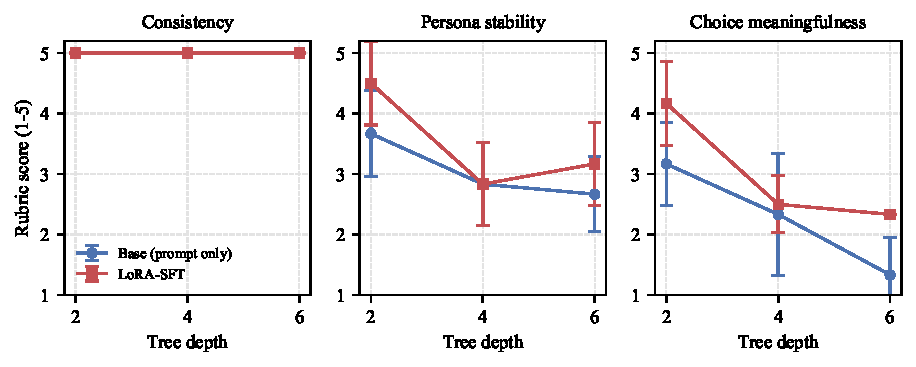
\includegraphics[width=\linewidth]{../experiment/plots/fig1_quality_depth.pdf}
\caption{Rubric scores versus tree depth (mean $\pm$ s.d.\ over eight trees per point).}
\label{fig:quality}
\end{figure}

\begin{table}[t]\centering\small
\caption{Rubric scores (1--5, mean $\pm$ s.d., $n=8$ per cell).}
\label{tab:rubric}
\begin{tabular}{llcccc}
\toprule
System & Depth & Consistency & Persona & Choice & Composite\\
\midrule
Base & 2 & 5.00$\pm$0.00 & 3.67$\pm$0.71 & 3.17$\pm$0.69 & 3.94\\
     & 4 & 5.00$\pm$0.00 & 2.83$\pm$0.69 & 2.33$\pm$1.01 & 3.39\\
     & 6 & 5.00$\pm$0.00 & 2.67$\pm$0.62 & 1.33$\pm$0.62 & 3.00\\
\midrule
LoRA & 2 & 5.00$\pm$0.00 & 4.50$\pm$0.69 & 4.17$\pm$0.69 & 4.56\\
     & 4 & 5.00$\pm$0.00 & 2.83$\pm$0.69 & 2.50$\pm$0.47 & 3.44\\
     & 6 & 5.00$\pm$0.00 & 3.17$\pm$0.69 & 2.33$\pm$0.00 & 3.50\\
\bottomrule
\end{tabular}
\end{table}

Table~\ref{tab:rubric} and Fig.~\ref{fig:quality} report the three scales and their mean as a
function of depth. For the prompt-only system the composite score falls from 3.94 at depth 2 to
3.39 at depth 4 and 3.00 at depth 6, a 24\% loss. The decline is not shared equally by the three
scales. Consistency is 5.00 in all 48 trees, because none of its three checks---fact conflict,
cross-world proper noun, out-of-world term---fires anywhere (the heuristic fact-conflict count is
zero in every cell). Persona stability loses 0.83 points between depth 2 and 4
(3.67$\to$2.83, $p=0.034$, exact Wilcoxon, $n=8$) and then stays flat (2.67 at depth 6). Choice
meaningfulness is the most depth-sensitive scale, falling at every step from 3.17 to 2.33 to 1.33,
a 58\% loss ($p=0.039$, $\Delta=1.00$ for depth $4\to6$).

LoRA-SFT changes the profile rather than lifting it uniformly. At depth 2 it gains on both soft
scales (persona 4.50, choice 4.17, composite 4.56, each $p=0.008$ against its own depth-4 level)
and beats the baseline on choice by a full point ($p=0.041$). At depth 4 the two systems are
statistically indistinguishable (3.44 versus 3.39). At depth 6 the adapter is ahead again (3.50
versus 3.00, choice $+1.00$, $p=0.014$), but the composition of that score has changed: persona
recovers to 3.17 while choice contributes exactly 2.33 with zero variance across all eight trees,
i.e.\ the same two of three checks fail in every single tree. The next subsection shows which.

\subsection{Structural Degradation}
\label{sec:structure}
\begin{figure}[t]\centering
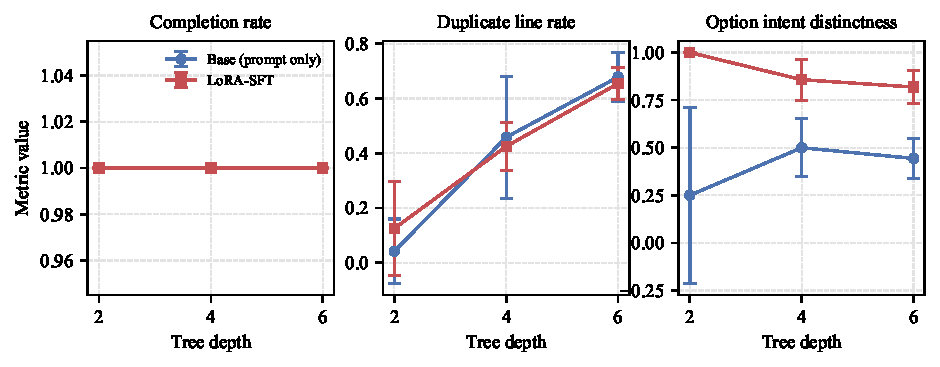
\includegraphics[width=\linewidth]{../experiment/plots/fig2_structure_depth.pdf}
\caption{Surface diversity and option metrics versus tree depth.}
\label{fig:structure}
\end{figure}

\begin{table}[t]\centering\small
\caption{Structural and option metrics (means, $n=8$ per cell). Num.\ drift counts invented
numerals per tree; time is seconds per tree.}
\label{tab:structure}
\begin{tabular}{llcccccc}
\toprule
System & $d$ & Dup line & Dist-2 & Intent dist. & Opt.\ dup & Pers.\ hit & Num.\ drift\\
\midrule
Base & 2 & 0.042 & 0.941 & 0.250 & 0.000 & 0.083 & 0.38\\
     & 4 & 0.458 & 0.479 & 0.500 & 0.098 & 0.142 & 0.63\\
     & 6 & 0.679 & 0.215 & 0.444 & 0.270 & 0.181 & 0.50\\
\midrule
LoRA & 2 & 0.125 & 0.875 & 1.000 & 0.000 & 0.583 & 1.00\\
     & 4 & 0.425 & 0.529 & 0.857 & 0.259 & 0.308 & 3.25\\
     & 6 & 0.655 & 0.270 & 0.819 & 0.659 & 0.315 & 14.88\\
\bottomrule
\end{tabular}
\end{table}

Fig.~\ref{fig:structure} and Table~\ref{tab:structure} show what depth does to the surface of the
text. Duplicate-line rate rises monotonically in both systems (base 0.04$\to$0.46$\to$0.68,
$p=0.018$ then $p=0.008$; adapter 0.13$\to$0.43$\to$0.66), and distinct-2 falls correspondingly
(0.94$\to$0.22 for the baseline), so the loss of novelty is not an artefact of a single metric:
the deep levels are largely recomposed from sentences already used elsewhere in the same tree.
Register hits move in the opposite direction for the baseline (0.08 at depth 2, 0.18 at depth 6),
but every value stays far below the 0.30 threshold, whereas the adapter starts high (0.58,
$p=0.023$ versus base) and decays to 0.31.

Option quality separates the two systems most sharply. Option-intent distinctness is
0.25/0.50/0.44 for the baseline and 1.00/0.86/0.82 for the adapter ($p\le0.014$ at all three
depths): the adapter does teach the model to keep the two branches semantically different. But it
collapses in the other direction. Its option-duplication rate grows from 0.00 to 0.26 to 0.66 and
at depth 6 is 2.4 times the baseline's 0.27 ($p=0.016$); inspecting the trees, a handful of generic
probes (``and then what happened that day?'') are reused across unrelated nodes. The adapter also
invents numbers: 1.0, 3.3 and 14.9 numerals per tree at depths 2, 4 and 6, against 0.4--0.6 for
the baseline. Both effects are what a template learned from silver data would predict: the model
has learned how options are shaped, not what this particular NPC would make the player choose.

Structural legality itself is intact in all 48 level-wise trees (completion 1.00, depth 1.00,
48/48 valid), which is the point of moving the topology into the harness. Time grows with the
number of calls (3, 15, 63 nodes): 14, 69 and 291 seconds for the baseline and 21, 80 and 335
seconds for the adapter, i.e.\ roughly 4--5 seconds per node on the 8\,GB laptop.

\subsection{One-shot versus Level-wise Generation}
\begin{figure}[t]\centering
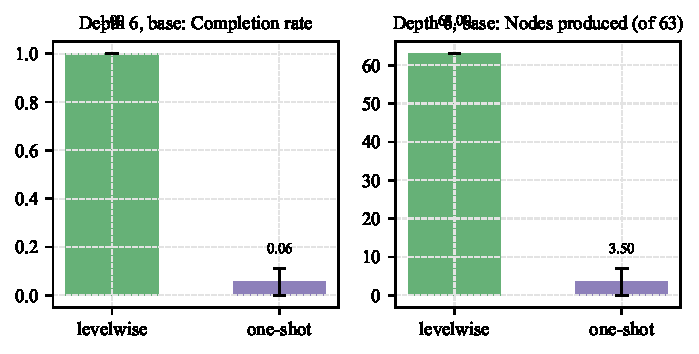
\includegraphics[width=\linewidth]{../experiment/plots/fig4_ablation_oneshot.pdf}
\caption{Depth-6 trees under both strategies (base model, first two worlds, seed 42). A single
call collapses structurally.}
\label{fig:ablation}
\end{figure}

The one-call strategy never produced a usable tree: 1 of 63 nodes for the first world and 6 of 63
for the second (completion 0.016 and 0.095), 0/2 structurally valid, after 37 and 23 seconds
(Fig.~\ref{fig:ablation}). The token budget was not the constraint---the call was allowed 7168 new
tokens, about 110 per expected node---and the model terminated on its own after the root, and after
one side branch in the second world. We deliberately do not report quality scores for these two
runs: the executor would score the fragments 4.11 and 3.67, and a one-node tree is trivially easy
to keep consistent. That is exactly the failure mode that a per-tree average hides and that a
structural comparison exposes: at depth 6, the whole-tree prompt does not produce a small tree, it
produces almost no tree.

\subsection{Trade-off Summary}
\begin{figure}[t]\centering
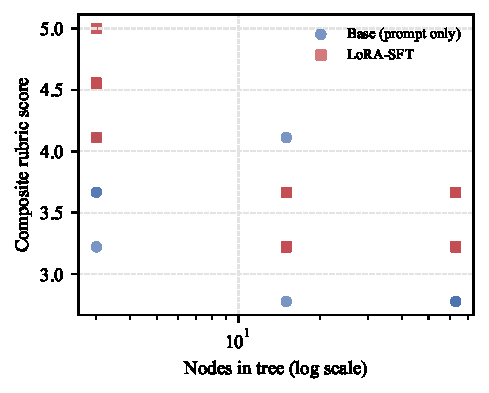
\includegraphics[width=\linewidth]{../experiment/plots/fig3_tradeoff.pdf}
\caption{Tree size versus composite rubric score (each point is one tree).}
\label{fig:tradeoff}
\end{figure}

Fig.~\ref{fig:tradeoff} plots composite score against tree size. Because the node count grows as
$2^{d}$, two extra levels multiply both authoring and inference cost by 4.2, while the baseline
composite drops by 0.94 points and the adapter's by 1.06 when going from depth 2 to depth 6.
Neither system recovers that loss at depth; the adapter is better at every depth except
depth 4, where the two are equal. For a 1.5B model the practical operating range is therefore
$d\le4$, and depth should be bought with concatenated shallow scenes or with human curation rather
than with a longer single tree.

\subsection{Qualitative Comparison}
Table~\ref{tab:paths} follows the first-option path of the same world and seed under both systems
(translated from Chinese). The baseline opens with a generic concern question, repeats it verbatim
at levels 3 and 5, and lets an option restate what the NPC itself just said (``I know you are short
of hands''), so the path never advances: the final line is still asking the player for help. The
adapter holds a dialogue-act arc (guarded, bargain, concede, deflect, reveal, reveal), and its leaf
delivers the world's concealed fact. Its failure is of a different kind: the option ``and then what
happened that day?'' is reused at levels 4 and 5, which is the option-duplication behaviour counted
in Table~\ref{tab:structure}.

\begin{table}[t]\centering\small
\caption{First-option path, ``Ash Chronicle'' (post-apocalyptic), $d=6$, seed 42. Translations by
the authors.}
\label{tab:paths}
\begin{tabular}{p{0.04\linewidth}p{0.42\linewidth}p{0.44\linewidth}}
\toprule
$d$ & Base (prompt only) & LoRA-SFT\\
\midrule
1 & You look nervous. Is something wrong? & Stop. In the Ash Chronicle, strangers state their business first.\\
2 & What are you talking about? I understand. & Let me be blunt: I want a return I can cash in immediately.\\
3 & You look nervous. Is something wrong? & Fine, since you did not use ash against me.\\
4 & I know you are short of hands. & I did not hear that.\\
5 & You look nervous. Is something wrong? & Thirty years of debt is not settled with an apology.\\
6 & I know you are short of hands; will you help? (leaf) & The surface they showed you is all screened. (leaf)\\
\bottomrule
\end{tabular}
\end{table}

\subsection{Judge Calibration}
\label{sec:judge-calib}
The base model was asked to apply the same rubric to 24 trees, depth-blind, three repetitions per
tree. It returned 5.0 on consistency, persona stability and choice meaningfulness for every tree
(variance 0 on all three scales), while the deterministic executor spans 2.78 to 5.00 on the same
sample. The correlation between the two is therefore undefined, not merely low. A 1.5B model in
this configuration does not execute a 1--5 rubric; it emits the ceiling. We report this as a
negative result, keep the judge run as a control, and rely on the deterministic executor plus the
released human-rating tool for measurement.

\subsection{Can Harness Interventions Recover the Loss?}
\label{sec:interventions}
The depth trend above leaves open whether the loss belongs to the task or to our pipeline. We
therefore built three deterministic interventions, none of which touches the weights, and re-ran
generation for $d\in\{2,4,6\}$ on the four evaluation worlds with seed 42, giving 24 paired trees
across the two systems. (i)~\emph{Beat sheet} (A1): a deterministic planner assigns every level a
content goal---which fact to advance, which level may unlock the secret---and only the current
level's goal is appended to that node's prompt line. (ii)~\emph{Dedupe resampling} (A2): a node whose
line or options exceed 0.90 character similarity to any previously emitted text, or that echoes the
player's last utterance, is resampled with an explicit blacklist, under a per-level budget of 60\% of
the node count. (iii)~\emph{Secret gating} (A4): the secret unlocks only at the deepest level, leaves
are forced into the reveal act, and a leaf that never touches the secret is rewritten once with the
secret stated in the prompt.

One negative result inside this intervention is worth reporting: an earlier variant that injected the
whole six-line beat sheet into every prompt \emph{lowered} the composite score of the same tree from
4.11 to 2.78, because output collapsed into short generic lines that dropped the NPC's own details.
Giving a 1.5B model a large block of global context does not make it plan; it makes it terse. Only the
per-node goal formulation helped.

\begin{table}[t]\centering\small
\caption{Harness interventions vs.\ the baseline pipeline (24 paired trees, seed 42). $\Delta>0$ means
the intervention scores higher. $p$: paired Wilcoxon over world$\times$depth$\times$system cells
($n=24$); entries with no variance are marked --.}
\label{tab:interventions}
\begin{tabular}{lcccc}
\toprule
Metric & v1 & +A1/A2/A4 & $\Delta$ & $p$\\
\midrule
Composite rubric & 3.704 & 3.907 & $+0.204$ & 0.048\\
Persona stability & 3.333 & 3.778 & $+0.445$ & 0.007\\
Persona grounding & 0.239 & 0.477 & $+0.238$ & $<0.001$\\
Duplicate-line rate & 0.365 & 0.312 & $-0.053$ & 0.069\\
Number hallucination & 3.125 & 2.208 & $-0.917$ & 0.058\\
Option-intent distinctness & 0.653 & 0.795 & $+0.142$ & 0.171\\
Choice meaningfulness & 2.778 & 2.944 & $+0.167$ & 0.666\\
Distinct-2 & 0.581 & 0.552 & $-0.028$ & 0.274\\
\midrule
Composite, $d=2$ & 4.389 & 4.500 & $+0.111$ & --\\
Composite, $d=4$ & 3.500 & 3.722 & $+0.222$ & --\\
Composite, $d=6$ & 3.222 & 3.500 & $+0.278$ & --\\
\bottomrule
\end{tabular}
\end{table}

Three observations follow. First, the gain grows with depth ($+0.11$, $+0.22$, $+0.28$): the harness
helps precisely where the baseline collapses, which supports reading part of the depth penalty as a
prompt-organisation artefact rather than a pure capability ceiling. Second, grounding is the largest
effect ($+0.238$, $p<0.001$): with a per-level content goal the NPC mentions its own possessions,
history and role instead of emitting generic lines, and persona stability rises accordingly
($+0.445$). Third, repetition barely moves. At $d=6$ the dedupe loop fired 34.1 times per tree but
repaired only 4.9 nodes, leaves touched the secret in 10--21\% of cases, and the cost was $+67\%$
model calls. A 1.5B model told not to repeat a sentence usually repeats it as a paraphrase, so surface
resampling cannot substitute for planning capacity. We therefore adopt A1, report A2/A4 as partial,
and treat the residual gap as evidence for the training-side remedies in
Section~\ref{sec:limits}.

\section{Discussion}
\subsection{Depth erodes variety and agency, not facts}
The clearest pattern in our data is that the three scales age very differently. Fact-level
consistency never moves, while surface novelty, register and option quality all degrade. One
reading is optimistic---a 1.5B model with a local prompt does not corrupt the world's facts---and
one is pessimistic: our consistency operationalisation only detects hard contradictions with the
fact list, cross-world proper nouns and out-of-world terms, all of which are easy for a model that
simply does not mention many facts. A deeper tree gives the model more chances to contradict
itself, but also more places to stay silent. We therefore read the flat 5.00 as \emph{saturation of
the check}, not as evidence that consistency is depth-invariant, and we flag attribute-level
consistency probing as the main measurement to add next (Section~\ref{sec:limits}).

\subsection{Choice meaningfulness is the binding constraint}
Choice meaningfulness loses 58\% between depth 2 and depth 6 in the baseline and is the only scale
that falls at both depth steps. The mechanism is visible in the trees: as the path grows, the
branching budget is spent on paraphrases (``tell me'' / ``tell me more''), and the baseline's
options frequently restate the NPC's own preceding line (Table~\ref{tab:paths}, level 4). Two of the
three checks that define the scale---option repetition and intent recognisability---are exactly the
ones the baseline fails, and they are the ones a designer would notice first when playing. If a
project can only afford to optimise one thing, this is it.

\subsection{Fine-tuning teaches form, not planning}
The adapter is a strong intervention at depth 2 (composite 4.56 versus 3.94, option-intent
distinctness 1.00 versus 0.25) and a wash at depth 4 (3.44 versus 3.39). Its training signal is a
set of 1600 independent node expansions: each pair teaches the output contract, the two-option
shape, register and length, but nothing in it requires coordinating a 63-node plan. Depth is
precisely the regime where the missing skill matters, which explains why the gain is concentrated
where the task is local. The side effects point the same way: the adapter learned that options
should look like short probes, and so it reuses a handful of them at depth 6 (duplication 0.66), and
it learned that in-world speech contains concrete quantities, and so it invents them (14.9
numerals per tree). Both are properties of the corpus, faithfully copied---a reminder that silver
data teaches style faster than judgement.

\subsection{Where the constraint lives matters more than model size}
The ablation is the most actionable result. With the same 1.5B model, the same prompt content and a
token budget of 7168, asking for the tree in one call yields 1 and 6 of 63 nodes; asking for one
node at a time, 63 times, yields 48/48 valid trees. Nothing about the model changed. The practical
implication for small studios is that the topology should be owned by the harness, with the model
used as a local text realiser, and that a planning step (our dialogue-act layer) is what keeps the
local calls from collapsing into the same sentence. It also implies an evaluation rule: per-tree
averages hide structural failure, because a tree that does not exist cannot score badly. Completion
rate and validity must be reported before any quality scale.

\section{Limitations and Ethics}
\label{sec:limits}
\textbf{Statistical resolution.} Two seeds give $n=8$ paired comparisons per test, whose smallest
attainable $p$-value is 0.0078; effects below roughly one rubric point are not resolvable, and the
depth-4 tie between systems should be read as ``no detectable difference'', not as equivalence. The
intervention comparison in Section~\ref{sec:interventions} uses a single seed and 24 cells, so its
$p$-values should be read as exploratory; a single tree's composite score varies by up to 0.9 across
samples of the same configuration, and we observed that variance directly when probing prompt variants.

\textbf{Measurement.} The rubric executor is a deterministic proxy with thresholds fixed by us
(duplicate rate below 0.10, register hits at least 0.30, option repetition below 0.05, intent
coverage at least 0.80). It cannot judge wit, dramatic timing or narrative payoff, and the
consistency scale saturates at 5.00. Human ratings have not yet been collected at a scale that
would support an agreement coefficient; the browser tool is released so that this can be done, and
until then no human-validated claim is made.

\textbf{External validity.} One model size (1.5B), four Chinese worlds with a single NPC each,
binary branching, and a programmatically generated training corpus. The template collapse we
observe may partly be inherited from that corpus; a larger model, or human-written silver data,
could behave differently. The one-shot ablation is an existence proof on two trees, not an
estimate of failure rate.

\textbf{Ethics.} No human subjects or personal data were involved. Generated dialogue can reproduce
biases of the base model, and our worlds include violence-adjacent themes; the demo is a research
prototype and any deployment needs content review. All prompts and per-tree records are archived so
that every number in this paper can be traced to a JSON file, and the negative judge result is
reported rather than discarded.

\section{Conclusion}
We asked whether a local 1.5B model can generate branching NPC dialogue trees, and how quality
trades off against depth. With the tree topology owned by the harness, the answer to the first
question is yes: 48/48 trees are structurally valid at depths 2, 4 and 6, while a single-call
baseline produces almost nothing. The answer to the second is that depth is not uniformly harmful:
fact-level consistency stays at its ceiling, but choice meaningfulness falls by 58\% and persona
stability by 27\% between depth 2 and 6, so a stronger tree is not automatically a better one. A
LoRA adapter trained on structure-aligned silver data removes most of the shallow-depth deficit and
still helps at depth 6, but at the cost of option template collapse and invented quantities. A third
result is that part of the depth penalty is organisational rather than intrinsic: appending a
per-level content goal to each node lifts the composite score from 3.70 to 3.91 and grounding from
0.24 to 0.48, and the benefit is largest at depth 6, whereas resampling repeated lines repairs only a
seventh of the cases it detects. Three methodological takeaways follow: enforce structure in the
harness rather than in the prompt, keep per-call prompts short and local even when the tree is long,
and do not delegate rubric scoring to a model of this size---it returns the ceiling for everything.

\bibliographystyle{IEEEtran}
\bibliography{refs}

\end{document}
